\chapter{Resultados}\label{chapter:results}

En este capítulo se presentan y analizan los resultados obtenidos a partir de la aplicación de los experimentos propuestos en capítulos anteriores. Se exponen las métricas estadísticas calculadas para cada grupo de experimentos, identificando las configuraciones que han demostrado el mejor desempeño. Asimismo, se realiza una comparación entre los resultados más destacados de cada grupo experimental. Finalmente, se incluye una evaluación cualitativa realizada por una especialista del área médica, complementada con el correspondiente análisis estadístico, con el objetivo de validar la relevancia y aplicabilidad de los hallazgos en el contexto clínico.

\section{Mejores resultados por grupos de experimentos}

\subsection{Mejora de energía}

En todos los experimentos realizados empleando la técnica de mejora de energía (véase la Tabla~\ref{tab:metricas}), no se observaron diferencias estadísticamente significativas entre los resultados obtenidos ($p > 0.05$). Esta ausencia de significancia se mantiene tanto al aplicar el preprocesamiento de normalización como al utilizar la extracción de ventana de valores. Cabe destacar que el preprocesamiento es necesario para reducir el rango de valores de la imagen, lo que permite que el procesamiento experimental se realice en un tiempo razonable. Por lo tanto, debe aplicarse dicho preprocesamiento independientemente de su impacto en la significancia estadística de los resultados.

Sin embargo, se seleccionó el resultado correspondiente al parámetro de mejora de energía igual a 10 (Figuras/*~\ref{fig:boxplot-enhancement} y \ref{fig:comparison-enhancement}), ya que esta configuración presentó los mejores tiempos de ejecución, con una ventaja promedio de 15 segundos entre todas las evaluadas, lo que resulta especialmente relevante para aplicaciones prácticas donde la eficiencia computacional es prioritaria.

\begin{figure}[H]
    \centering
    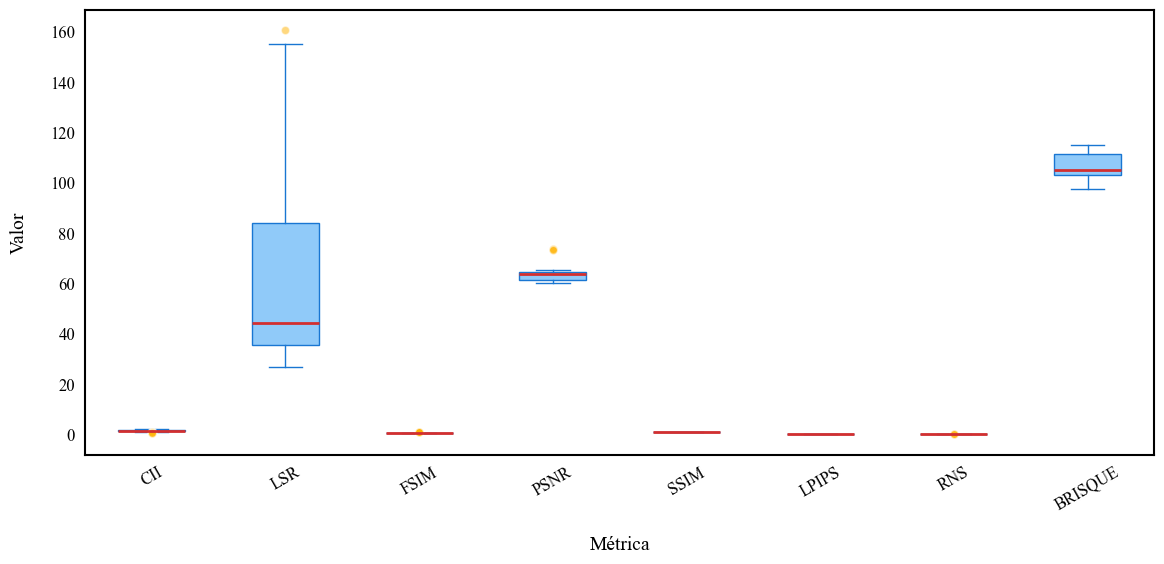
\includegraphics[width=0.95\textwidth]{Graphics/boxplot-enhancement.png}
    \caption{Gráfico de cajas y bigotes de los valores de las métricas para el experimento Mejora de energía con parámetro 10.}
    \label{fig:boxplot-enhancement}
\end{figure}

\begin{figure}[H]
    \centering
    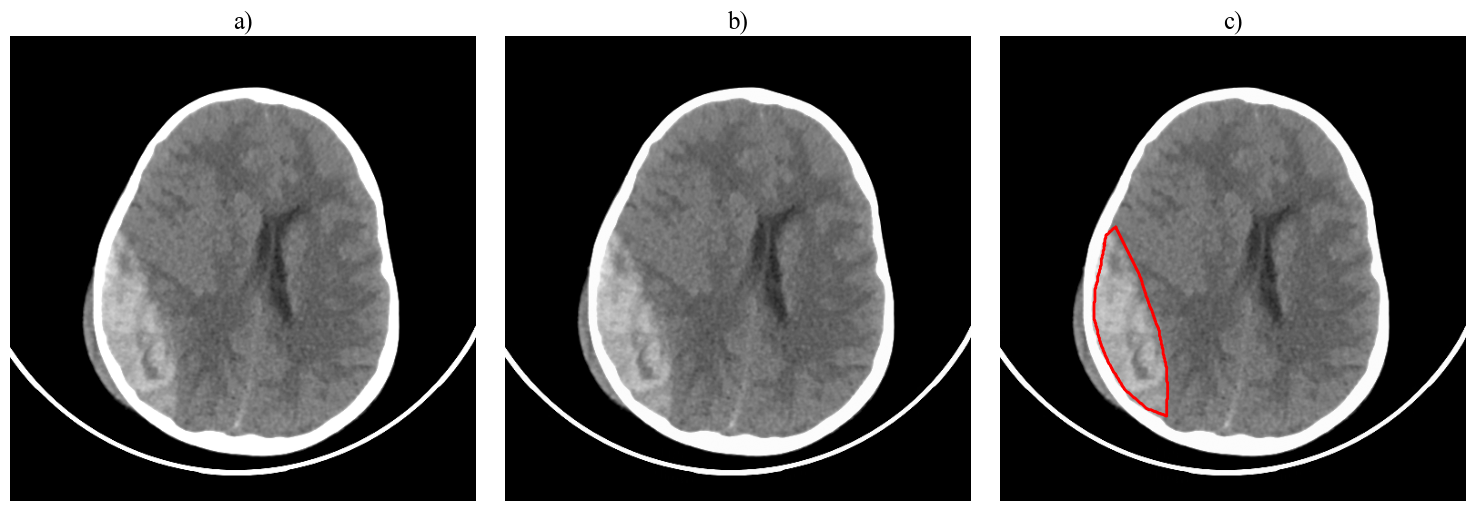
\includegraphics[width=0.95\textwidth]{Graphics/comparison-enhancement.png}
    \caption{Comparación de a) imagen original, b) imagen modificada, c) imagen modificada con la lesión destacada.}
    \label{fig:comparison-enhancement}
\end{figure}

\subsection{Umbralización}

En todos los experimentos realizados empleando la técnica de umbralización (véase la Tabla~\ref{tab:metricas}), no se observaron diferencias estadísticamente significativas entre los resultados obtenidos ($p > 0.05$). Esta ausencia de significancia se mantiene tanto al aplicar el preprocesamiento de normalización como al utilizar la extracción de ventana de valores.

Sin embargo, se seleccionó el resultado correspondiente al umbral de 0.001 (Figuras/*~\ref{fig:boxplot-threshold} y \ref{fig:comparison-thresholding}), ya que esta configuración presentó los mejores tiempos de ejecución, con una ventaja promedio de 4 segundos entre todas las evaluadas, lo que resulta especialmente relevante para aplicaciones prácticas donde la eficiencia computacional es prioritaria.

\begin{figure}[H]
    \centering
    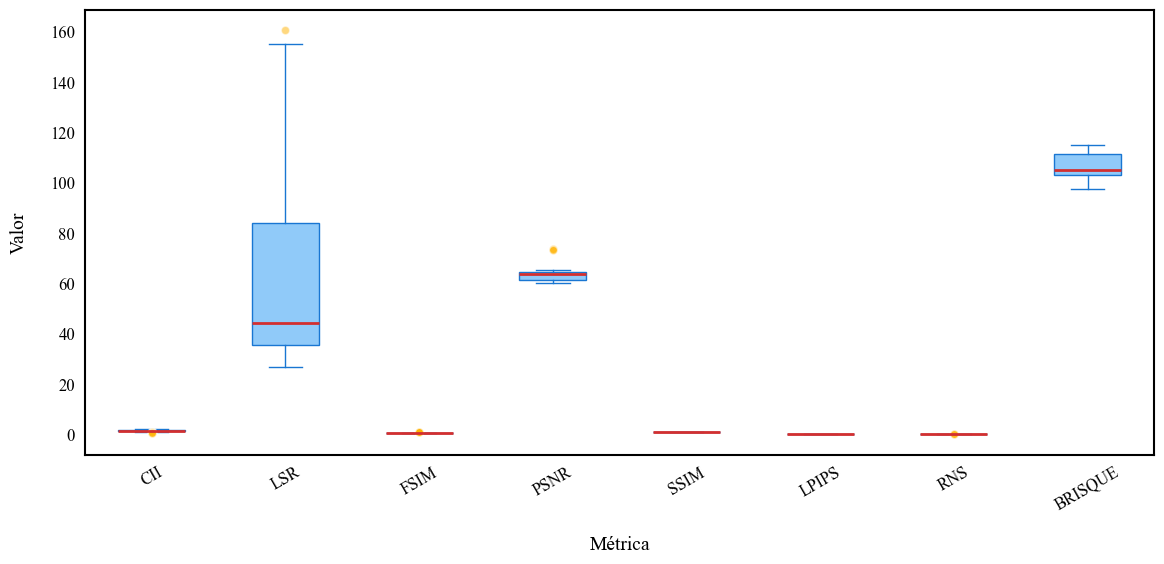
\includegraphics[width=0.95\textwidth]{Graphics/boxplot-threshold.png}
    \caption{Gráfico de cajas y bigotes de los valores de las métricas para el experimento Umbralización con parámetro 0.001.}
    \label{fig:boxplot-threshold}
\end{figure}

\begin{figure}[H]
    \centering
    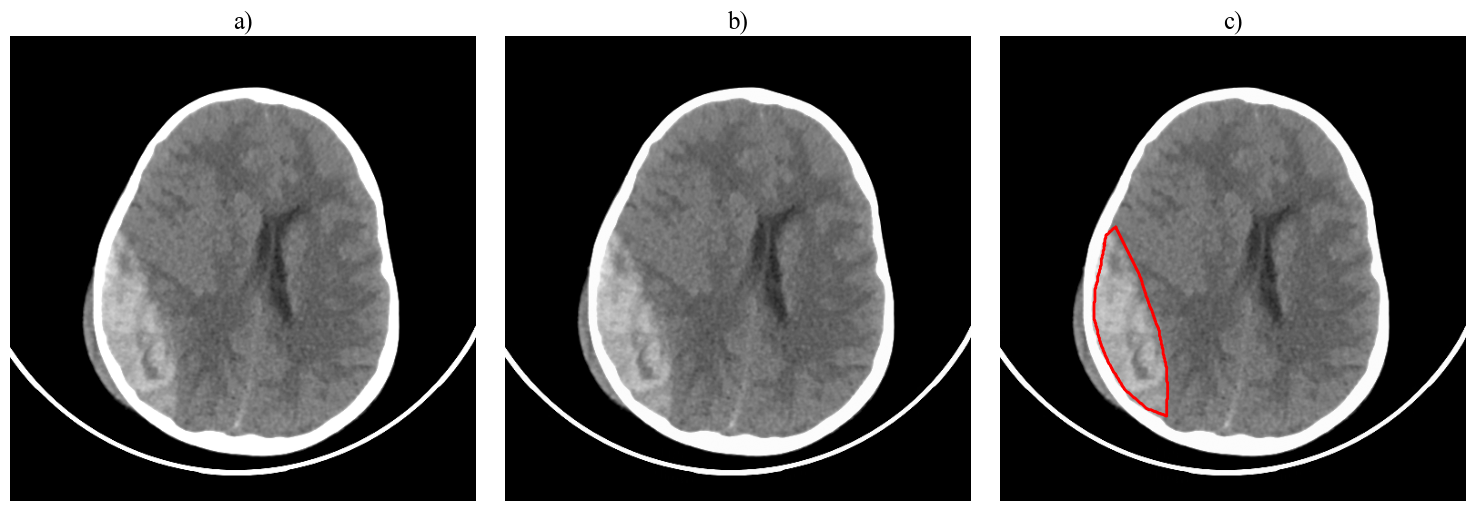
\includegraphics[width=0.95\textwidth]{Graphics/comparison-thresholding.png}
    \caption{Comparación de a) imagen original, b) imagen modificada, c) imagen modificada con la lesión destacada.}
    \label{fig:comparison-thresholding}
\end{figure}

\subsection{Máscara de paso alto}

Para evaluar el impacto de los diferentes parámetros en el filtrado de paso alto, se empleó la métrica BRISQUE, que permite estimar la calidad de imagen de manera automática y sin referencia, asignando puntuaciones donde valores más bajos indican mejor calidad percibida \cite{BRISQUE}. En este contexto, se compararon dos configuraciones del filtro pasa alto, utilizando valores de \texttt{cutoff\_scale} de 5 y 10.

Los resultados obtenidos muestran que la configuración con \texttt{cutoff\_scale} igual a 5 alcanzó una puntuación BRISQUE de 108.93, mientras que la configuración con \texttt{cutoff\_scale} igual a 10 obtuvo un valor de 110.90 (Figuras/*~\ref{fig:boxplot-highpass} y \ref{fig:comparison-highpass}). Dado que una menor puntuación BRISQUE indica una menor presencia de artefactos y, por tanto, una mejor calidad de imagen, se considera que la configuración con \texttt{cutoff\_scale} de 5 presenta un desempeño superior según esta métrica.

Cabe destacar que, aunque se evaluaron otras métricas de calidad, no se encontró suficiente evidencia estadística para afirmar que existan diferencias significativas entre ambas configuraciones en dichas métricas. Por lo tanto, la selección de la configuración óptima se fundamenta en los resultados obtenidos con BRISQUE, en concordancia con los criterios objetivos de evaluación empleados en este trabajo.

\begin{figure}[H]
    \centering
    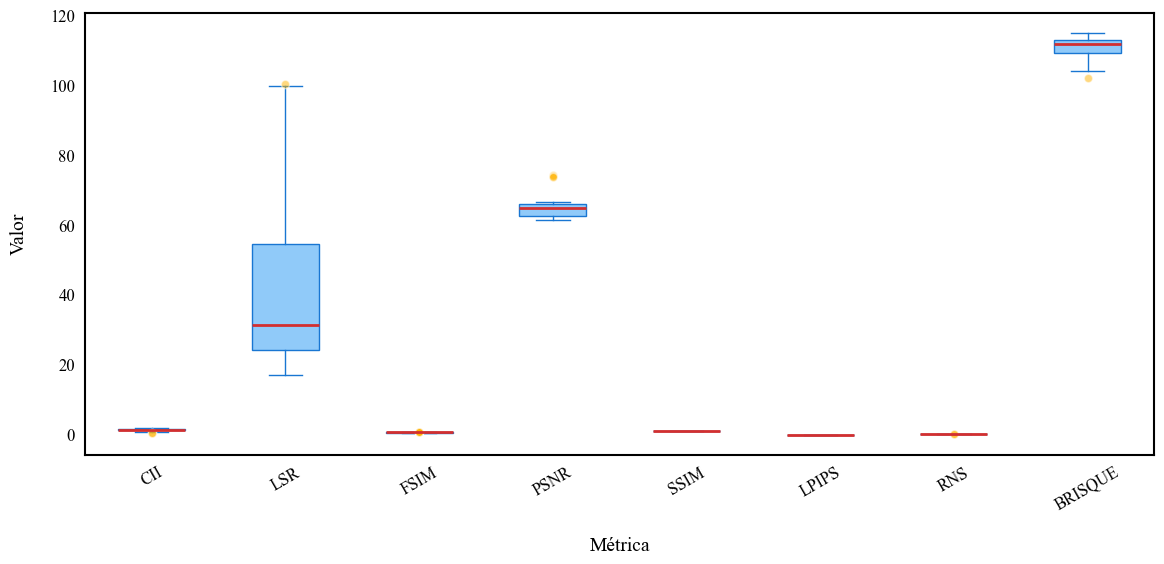
\includegraphics[width=0.95\textwidth]{Graphics/boxplot-highpass-mask.png}
    \caption{Gráfico de cajas y bigotes de los valores de las métricas para el experimento Máscara de paso alto con parámetros 5.}
    \label{fig:boxplot-highpass}
\end{figure}

\begin{figure}[H]
    \centering
    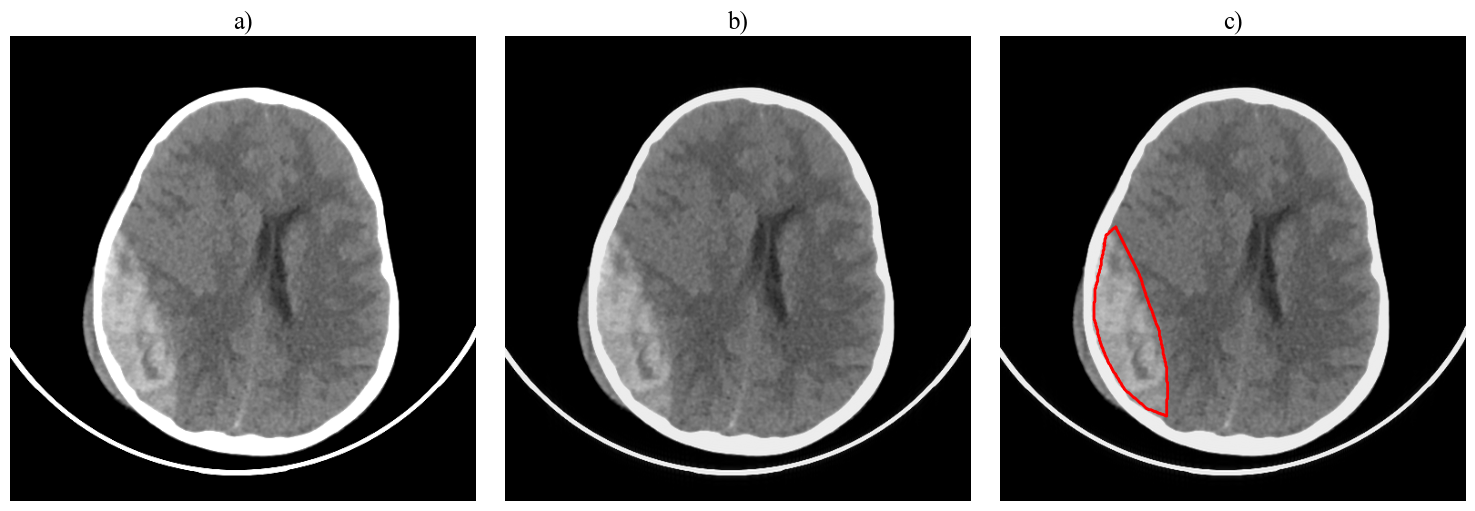
\includegraphics[width=0.95\textwidth]{Graphics/comparison-highpass.png}
    \caption{Comparación de a) imagen original, b) imagen modificada, c) imagen modificada con la lesión destacada.}
    \label{fig:comparison-highpass}
\end{figure}

\subsection{Máscara de pasa banda}

Para analizar el efecto de los parámetros en el filtrado pasa banda, se empleó la métrica LSR, que cuantifica el nivel de nitidez en la imagen mediante el análisis de bordes y detalles finos, siendo un indicador clave de la calidad visual en imágenes biomédicas. En este análisis, se compararon dos configuraciones de la máscara de pasa banda: \texttt{low\_scale=5, high\_scale=10} y \texttt{low\_scale=15, high\_scale=20}.

Los resultados indican que la configuración \textit{Máscara de pasa banda con low\_scale=5, high\_scale=10} obtuvo una puntuación LSR de 54.92, mientras que la configuración con \texttt{low\_scale=15, high\_scale=20} alcanzó un valor de 37.54 (Figuras/*~\ref{fig:boxplot-bandpass} y \ref{fig:comparison-bandpass}). Dado que un mayor valor de LSR refleja una mayor nitidez y, por ende, mejor calidad visual, se concluye que la primera configuración ofrece un desempeño superior según esta métrica.

Es importante señalar que, aunque se evaluaron otras métricas de calidad, no se encontró suficiente evidencia estadística para afirmar que existan diferencias significativas entre ambas configuraciones en dichas métricas. Por consiguiente, la selección de la configuración óptima se fundamenta en los resultados obtenidos con LSR, en línea con los criterios objetivos de evaluación adoptados en este estudio.

\begin{figure}[H]
    \centering
    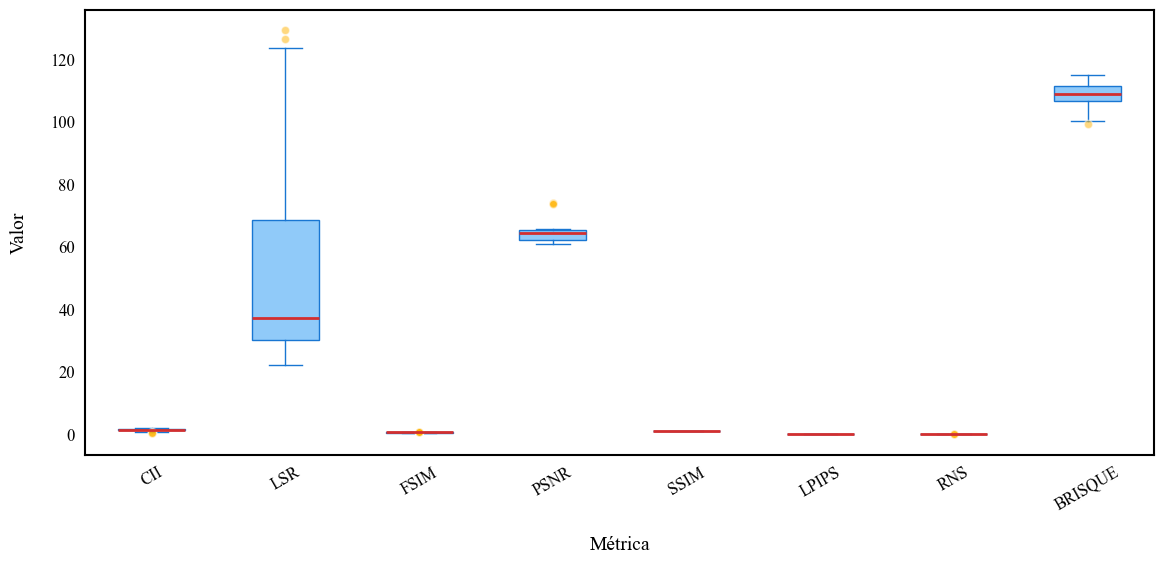
\includegraphics[width=0.95\textwidth]{Graphics/boxplot-bandpass-mask.png}
    \caption{Gráfico de cajas y bigotes de los valores de las métricas para el experimento \textit{Máscara de pasa banda con low\_scale=5, high\_scale=10}.}
    \label{fig:boxplot-bandpass}
\end{figure}

\begin{figure}[H]
    \centering
    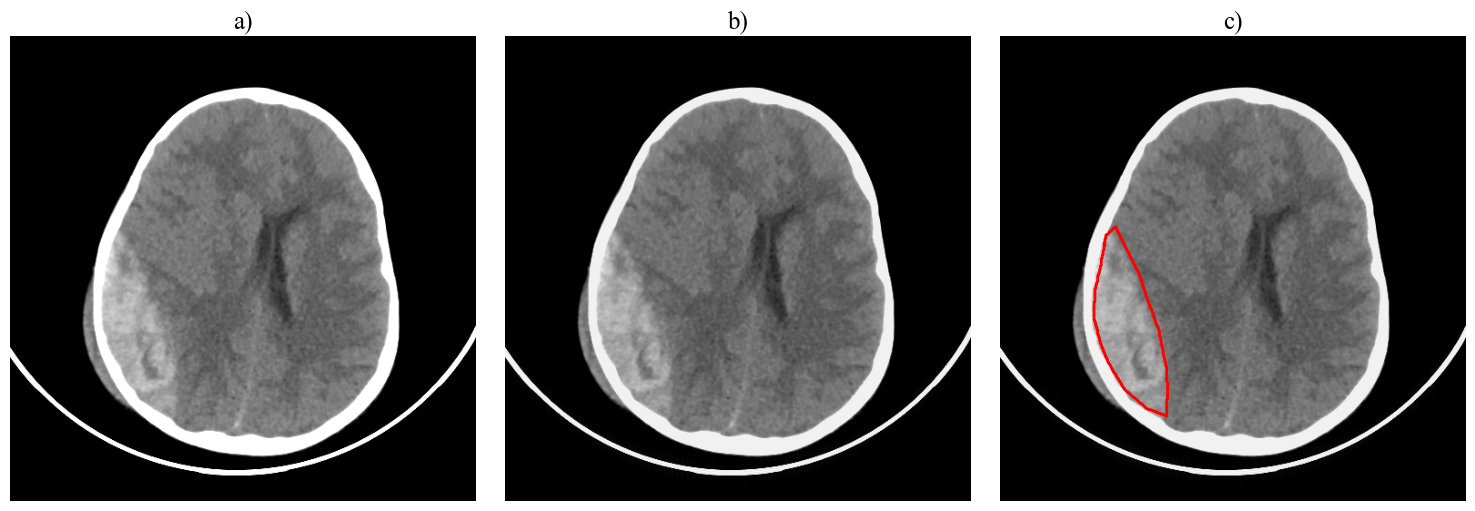
\includegraphics[width=0.95\textwidth]{Graphics/comparison-bandpass.png}
    \caption{Comparación de a) imagen original, b) imagen modificada, c) imagen modificada con la lesión destacada.}
    \label{fig:comparison-bandpass}
\end{figure}

\subsection{Máscara de escala exponencial}

En el análisis de la máscara de escala exponencial, se compararon dos configuraciones experimentales con valores de \texttt{decay\_rate} de 0.1 y 0.01. Los resultados muestran que ambas configuraciones son equivalentes en términos de las métricas de calidad evaluadas, ya que no se encontró suficiente evidencia estadística para afirmar que sus resultados sean diferentes.

Dado que la configuración con \texttt{decay\_rate} igual a 0.01 presentó un mejor desempeño en tiempos de ejecución en un promedio de 3.5 segundos, se selecciona esta opción como la más adecuada para aplicaciones donde la eficiencia computacional es prioritaria (Figuras/*~\ref{fig:boxplot-exponential} y \ref{fig:comparison-exponential}).

\begin{figure}[H]
    \centering
    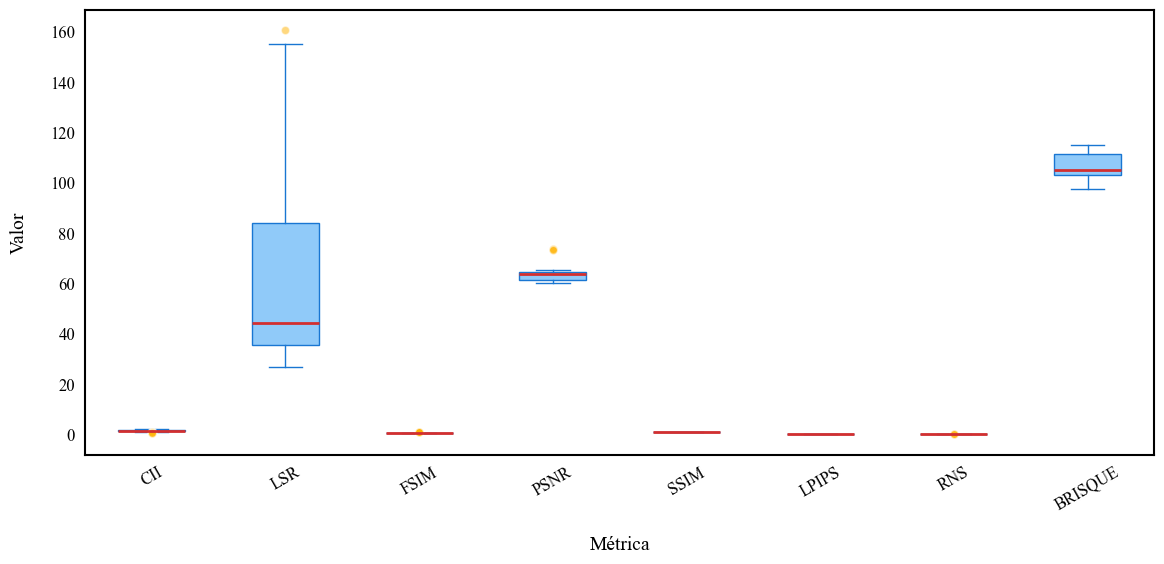
\includegraphics[width=0.95\textwidth]{Graphics/boxplot-exponential-mask.png}
    \caption{Gráfico de cajas y bigotes de los valores de las métricas para el experimento \textit{Máscara exponencial con decay\_rate=0.01}.}
    \label{fig:boxplot-exponential}
\end{figure}

\begin{figure}[H]
    \centering
    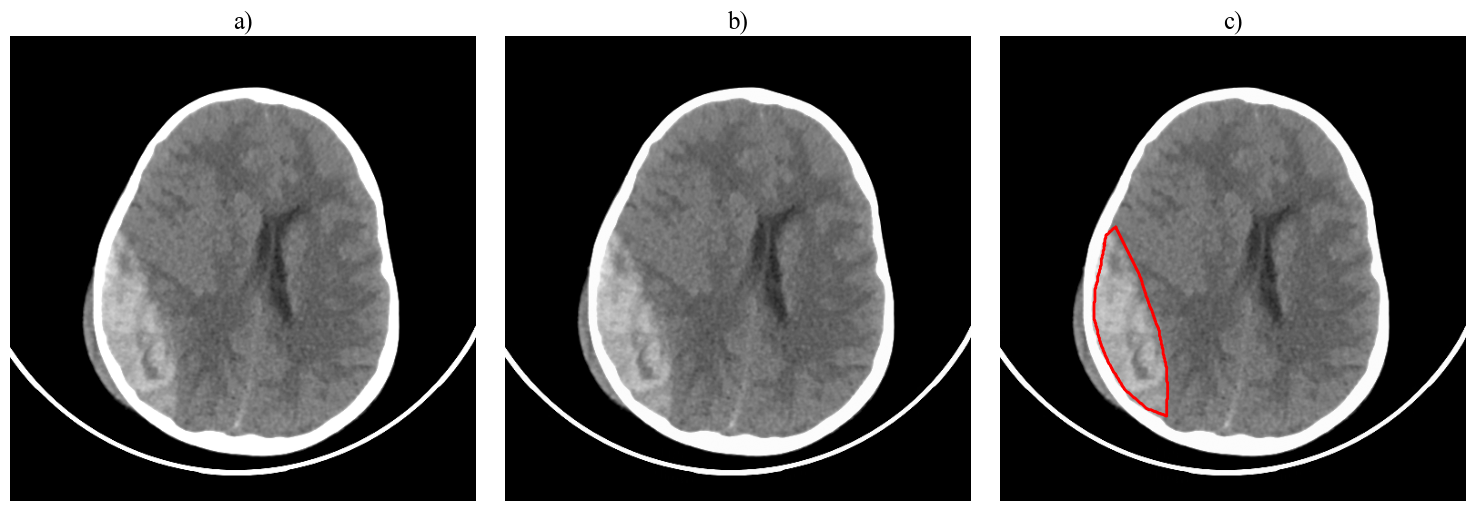
\includegraphics[width=0.95\textwidth]{Graphics/comparison-exponential.png}
    \caption{Comparación de a) imagen original, b) imagen modificada, c) imagen modificada con la lesión destacada.}
    \label{fig:comparison-exponential}
\end{figure}

\subsection{Máscara de escala gaussiana}

Se evaluaron tres configuraciones de la máscara de escala gaussiana, variando el parámetro \texttt{sigma} en valores de 1.0, 4.0 y 6.0, manteniendo \texttt{center\_scale=N/2}. Los resultados muestran que las configuraciones con \texttt{sigma=4.0} y \texttt{sigma=6.0} son equivalentes en términos de las métricas de calidad evaluadas, sin diferencias estadísticamente significativas.

Sin embargo, la configuración con \texttt{sigma=1.0} superó a las demás en la mayoría de las métricas relevantes, incluyendo CII, LSR, PSNR, SSIM, LPIPS y RNS, lo que indica una mejor calidad de imagen y menor distorsión. Por tanto, se selecciona la máscara de escala gaussiana con \texttt{center\_scale=N/2, sigma=1.0} como la opción óptima para este grupo experimental, en concordancia con los criterios objetivos de evaluación empleados en este trabajo.

\begin{figure}[H]
    \centering
    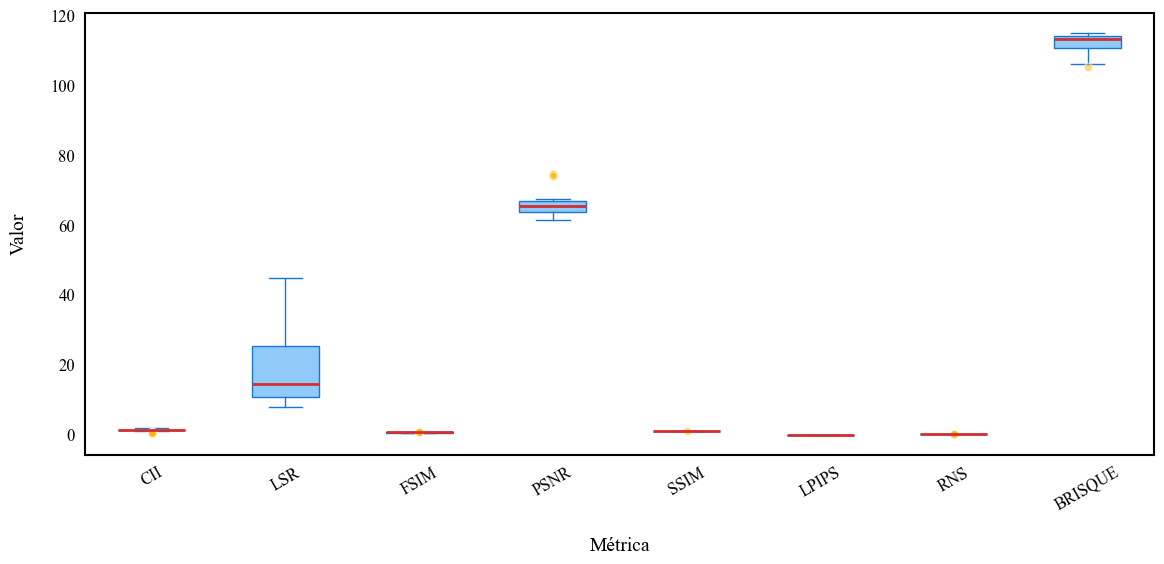
\includegraphics[width=0.95\textwidth]{Graphics/boxplot-gaussian-mask.png}
    \caption{Gráfico de cajas y bigotes de los valores de las métricas para el experimento \textit{Máscara de pasa banda con $\mu = N/2$, $\delta=1$}.}
    \label{fig:boxplot-gaussian}
\end{figure}

\begin{table}[H]
    \centering
    \caption{Comparativa de métricas para las configuraciones de la máscara de escala gaussiana (\texttt{center\_scale=N/2}).}
    \begin{tabular}{|l|c|c|c|}
    \hline
    \textbf{Métrica} & \textbf{sigma=1.0} & \textbf{sigma=4.0} & \textbf{sigma=6.0} \\
    \hline
    CII & 1.2515 & 1.4690 & 1.4690 \\
    LSR & 19.2774 & 67.1471 & 67.1471 \\
    FSIM & 0.6382 & 0.6181 & 0.6181 \\
    PSNR & 65.7315 & 63.7677 & 63.7677 \\
    SSIM & 0.9976 & 0.9963 & 0.9963 \\
    LPIPS & 0.0002 & 0.0004 & 0.0004 \\
    RNS & 0.1129 & 0.1405 & 0.1405 \\
    BRISQUE & 111.9635 & 106.8134 & 106.8134 \\
    \hline
    \end{tabular}
    \label{tab:gaussian_comparativa}
\end{table}

\section{Selección del mejor modelo}

El proceso de selección del mejor modelo se realizó a partir de una comparación entre los experimentos que obtuvieron los mejores resultados en cada una de las categorías evaluadas: umbralización, máscaras exponenciales y gaussianas, filtros pasa alto y pasa banda, así como la mejora de energía. Para garantizar una evaluación objetiva y exhaustiva se emplearon múltiples métricas de calidad de imagen, incluyendo FSIM, LSR, BRISQUE, PSNR, SSIM, LPIPS y RNS, cubriendo aspectos de nitidez, distorsión, artefactos y similitud estructural.

En la primera etapa se identificaron los experimentos con mejor desempeño dentro de cada grupo, seleccionando los siguientes: \textit{Threshold Coefficients at 0.001}, \textit{Exponential Scale Mask with decay\_rate=0.01}, \textit{Highpass Mask with cutoff\_scale=10}, \textit{Gaussian Scale Mask with center\_scale=N/2, sigma=1.0}, \textit{Bandpass Mask with low\_scale=5, high\_scale=10} y \textit{Enhance Energy by 10}.

Posteriormente, se realizó una comparación cruzada entre estos modelos. Los resultados mostraron que varias configuraciones, como la umbralización y la mejora de energía, presentaron desempeños equivalentes en la mayoría de las métricas evaluadas, sin diferencias estadísticamente significativas. Sin embargo, a medida que se avanzó en la comparación directa con los otros métodos, emergieron diferencias claras en métricas clave.

La máscara gaussiana con \texttt{center\_scale=N/2, sigma=1.0} destacó consistentemente sobre las demás configuraciones. Superó a los otros modelos en métricas como LSR (67.15 frente a valores significativamente menores en otros métodos), PSNR (65.73), SSIM (0.9976), LPIPS (0.00021), y RNS (0.1129), lo que indica una mayor nitidez, menor distorsión y mejor preservación de la estructura y los detalles de la imagen. Además, aunque en la métrica BRISQUE no obtuvo el valor más bajo absoluto, su desempeño global en el conjunto de métricas fue superior.

Este proceso de selección evidencia la importancia de considerar múltiples dimensiones de calidad de imagen y no basar la decisión únicamente en una métrica aislada. Así, la \textit{Máscara de escala gaussiana con center\_scale=N/2, sigma=1.0} fue seleccionada como el mejor modelo global, al ofrecer el balance óptimo entre nitidez, preservación de detalles y baja distorsión, validando su aplicabilidad en el procesamiento avanzado de imágenes de CT cerebral.

\begin{table}[H]
\centering
\caption{Comparativa de métricas para los mejores modelos de cada categoría.}
\resizebox{\textwidth}{!}{
\begin{tabular}{|l|c|c|c|c|c|c|}
\hline
\textbf{Métrica} & \textbf{Umbral 0.001} & \textbf{Exp. 0.01} & \textbf{Pasa alto 10} & \textbf{Gaussiana 1.0} & \textbf{Pasa banda 5-10} & \textbf{Energía 10} \\
    \hline
    CII & 1.4690 & 1.4690 & 1.3364 & 1.2515 & 1.3950 & 1.4690 \\
    LSR & 67.1471 & 67.1471 & 43.4102 & 19.2774 & 54.9205 & 67.1471 \\
    FSIM & 0.6181 & 0.6181 & 0.6305 & 0.6382 & 0.6248 & 0.6181 \\
    PSNR & 63.7677 & 63.7677 & 64.9677 & 65.7315 & 64.4397 & 63.7677 \\
    SSIM & 0.9963 & 0.9963 & 0.9972 & 0.9976 & 0.9968 & 0.9963 \\
    LPIPS & 0.0004 & 0.0004 & 0.0003 & 0.0002 & 0.0003 & 0.0004 \\
    RNS & 0.1405 & 0.1405 & 0.1235 & 0.1129 & 0.1308 & 0.1405 \\
    BRISQUE & 106.8134 & 106.8134 & 110.8965 & 111.9635 & 108.9883 & 106.8134 \\
    \hline
\end{tabular}
}
\label{tab:comparativa_final}
\end{table}

\section{Comparación con otros métodos}

El objetivo de esta sección es realizar una comparación cuantitativa entre el modelo propuesto y otros enfoques recientes basados en IA. Para ello, se emplean las métricas PSNR y SSIM, reconocidas y utilizadas como estándar en la literatura para la evaluación de calidad de imagen en tareas de reconstrucción, mejora y reducción de ruido en CT.

La elección de PSNR y SSIM responde a su capacidad para proporcionar una evaluación objetiva y reproducible de la similitud y la fidelidad entre la imagen original y la imagen procesada. PSNR cuantifica la relación entre la señal y el ruido introducido, permitiendo comparar el nivel de distorsión global, mientras que SSIM evalúa la preservación de la estructura, el contraste y la luminancia, aspectos fundamentales para la interpretación clínica y la percepción visual de la calidad en imágenes médicas. Su uso generalizado en estudios comparativos facilita la interpretación de los resultados y la comparación directa con trabajos previos en el área \cite{ImageProcessingBook, wang2004image}.

\begin{table}[h]
    \centering
    \caption{Comparación cuantitativa de métodos de mejora de imágenes de CT según PSNR y SSIM.}
    \label{tab:metodos_vs_metricas}
    \begin{tabular}{|l|c|c|}
        \hline
        \textbf{Método} & \textbf{PSNR} & \textbf{SSIM} \\
        \hline
        Máscara gaussiana & 65.7315 & 0.9976 \\
        EDCNN             & 42.0835 & 0.9866 \\
        LEARN++           & 49.0300 & 0.9924 \\
        ULTRA             & 58.3400 & 0.9518 \\
        \hline
    \end{tabular}
\end{table}

En Tabla~\ref{tab:metodos_vs_metricas} se observan diferencias significativas en el desempeño de los distintos métodos. El modelo basado en máscara gaussiana obtiene los valores más altos tanto en PSNR como en SSIM, lo que indica una mayor fidelidad respecto a la imagen original y una mejor preservación de las estructuras relevantes en la imagen de CT. En comparación los métodos de IA EDCNN, LEARN++ y ULTRA presentan valores inferiores en ambas métricas, siendo EDCNN el que muestra el menor PSNR y SSIM entre los métodos evaluados.

Estos resultados evidencian que el enfoque propuesto no solo logra reducir la distorsión global de la imagen, sino que también mantiene la integridad estructural y perceptual, aspectos fundamentales para la interpretación clínica. El valor de PSNR refleja una menor cantidad de error introducido durante el proceso de mejora, mientras que el alto valor de SSIM confirma que las características estructurales y el contraste se preservan de manera efectiva~\cite{wang2004image,ImageProcessingBook,upcommonsSSIM2023}. En conjunto, estos indicadores respaldan la idoneidad del método propuesto frente a alternativas recientes basadas en inteligencia artificial.


\section{Evaluación cualitativa por especialista}

Con el objetivo de complementar el análisis cuantitativo y validar la relevancia clínica de los métodos propuestos, se realizó una evaluación cualitativa a través de una encuesta dirigida a una especialista en neorología. Para este fin, se seleccionaron imágenes mejoradas utilizando el mejor método identificado en la comparación cuantitativa (máscara gaussiana) y el método con menor desempeño (umbralización). El mejor y peor método se decidieron en base a las métricas PSNR y SSIM con el objetivo de priorizar la eliminación de ruido manteniendo una similaridad con la imagen original.

La encuesta diseñado en \texttt{Google Forms} \cite{encuesta2025} consistió en 32 pares de imágenes, cada par compuesto por una imagen mejorada con la máscara gaussiana y otra con el método de umbralización. Los pares fueron seleccionados aleatoriamente de distintas secciones del conjunto de datos, y el orden de presentación fue completamente aleatorio para evitar cualquier sesgo y garantizar que la especialista no pudiera identificar el método aplicado en cada caso (presentacion a doble ciego).

El evaluador en un doctor en medicina, especialista en primer grado de Neurología, Médico General Integral y con 20 años de experiencia en el tema.

Los resultados obtenidos revelaron que en 19 casos ambos métodos fueron considerados equivalentes por el evaluador. En 9 casos, el método de umbralización fue valorado como “mucho mejor” y, en 3 casos, la máscara gaussiana recibió dicha calificación.

Para analizar estadísticamente estas preferencias, se aplicó la prueba de McNemar, adecuada para comparar proporciones en datos pareados y determinar si existen diferencias significativas en la preferencia entre dos métodos \cite{mcnemar}. El valor del estadístico de McNemar fue $2.0833$, $p = 0.1489$. Según estos resultados, aunque se observó una preferencia por el método de umbralización en los casos discordantes ($50.0\%$ de diferencia), esta diferencia alcanzó significancia estadística, si se considera un $\alpha = 0.2$ permitido en el caso de muestras pequeñas.

Estos hallazgos sugieren que, desde la perspectiva cualitativa del especialista, se hallaron diferencias significativas en la percepción de calidad entre ambos métodos en el contexto evaluado.